\section{x-project toolkit}\label{sec:toolkit}

``Everything is an element'', from an AJAX request to an entire web page. Every part of the website is encapsulated inside an element. 

\brand{x-project} provide a set of Polymer element for local routing, API requests, forms, lists, and style, liste below \footnote{\scriptsize For the sake of conciseness, Polymer Elements are presented as empty elements, although empty element type is not supported. Furthermore, template variable are enclosed in single curly brackets while Polymer requires double curly brackets.}. 

Elements can be customized through their attributes. We note that attributes could acts as inputs parameters (values that have effects to the element) or output parameters (values that are returned by the element).
Values in parameters could be hard-coded (if they never change) or stored in variables.
Different parameters in different elements could use the same variable, so, the value of an output parameter of an element could be used as input in an input parameter of another element.

\paragraph{Elements for local routing}

The following elements performs local routing (for Single Page Application).

\vspace{0.2cm}

\texttt{<x-router>} implements local routing using \emph{HTML5 Push State API}. It represent the core element of the app. It intercepts routes, create pages, and pass parameters to the page.

\vspace{0.2cm}

\texttt{<x-route>} represents a route-to-page mapping. 
Parameters presented in an URL are sent as attributes to the corresponding page.

\begin{lstlisting}[language=HTML5]
<x-route route="{route}" page="{page}" />
\end{lstlisting}

\texttt{<x-link>} is an extension of the anchor element \texttt{<a>} that prevents the default behavior when a click event occurs, blocking page request to the server and redirecting the request to the local router. 

\begin{lstlisting}[language=HTML5]
<a is="x-link" href="{href}">{link}</a>
\end{lstlisting}

\paragraph{Elements for API management}

The following elements handle HTTP RESTful API for the collections of the app.

\texttt{<api-collection-schema>} gets the schema of a collection. 

\begin{lstlisting}[language=HTML5]
<api-collection-schema 
  name="{collection}" 
  schema="{schema}" />
\end{lstlisting}

\vspace{0.2cm}

\texttt{<api-collection-post>} create a model of a collection. 

\begin{lstlisting}[language=HTML5]
<api-collection-post 
  name="{name}" model="{model}" />
\end{lstlisting}

\vspace{0.2cm}

\texttt{<api-collection-get>} gets models of a collection. 

\begin{lstlisting}[language=HTML5]
<api-collection-get 
  name="{collection}" where="{where}" 
  page="{page}" perpage="{perpage}"  
  items="{items}" count="{count}" />
\end{lstlisting}

Where: 
\texttt{name} is the name of the collection to retrieve; 
\texttt{where} is an object that specifies a set of logical conditions to match, similar to a \texttt{WHERE} clause in a SQL query;
\texttt{page} and \texttt{perpage} are parameters for the pagination;
\texttt{items} are the retrieved models that match the query composed by the \texttt{where} and the pagination parameters;
\texttt{count} is the size of the collection (the number of items of the collection).

\vspace{0.2cm}

\texttt{<api-collection-where>} generate dinamically (from a model schema) a form to create an API \texttt{where} clause filter. Specifically, for each property described in the model schema, it generates a corresponding input field. 

\begin{lstlisting}[language=HTML5]
<api-collection-where 
  schema="{schema}"
  where="{where}" />
\end{lstlisting}

\texttt{<api-model-get>} retrieve a model of a collection. 

\begin{lstlisting}[language=HTML5]
<api-model-get 
  name="{name}" model-id="{id}" 
  model="{model}" />
\end{lstlisting}

Where: 
\texttt{name} is the name of the collection of the model; 
\texttt{model-id} is the model id; 
\texttt{model} is the model retrieved (it acts as an output).

\texttt{<api-model-put>} update a model of a collection. 

\begin{lstlisting}[language=HTML5]
<api-model-put 
  name="{name}" model-id="{id}" 
  model="{model}" />
\end{lstlisting}

Where: 
\texttt{model} is the model updated (it acts as an input).

\vspace{0.2cm}

\texttt{<api-model-del>} delete a model of a collection. 

\begin{lstlisting}[language=HTML5]
<api-model-del name="{name}" model-id="{id}" />
\end{lstlisting}

\paragraph{Elements for forms}
The following elements are used to create forms. 

\vspace{0.2cm}

\texttt{<x-input>} is an extension of the input element. 

\begin{lstlisting}[language=HTML5]
<x-input 
  type="{type}" label="{label}"
  value="{value}" />
\end{lstlisting}

Where: 
\texttt{type} can be \texttt{string}, \texttt{number}, \texttt{date}, \texttt{email}, \texttt{url}, \texttt{location} (with autocompletion based on Google Place API) and \texttt{file}.

\vspace{0.2cm}

\texttt{<x-form>} generate dinamically (from a model schema) a form to create/update a model.

\begin{lstlisting}[language=HTML5]
<x-form schema="{schema}" model="{model}" />
\end{lstlisting}

\paragraph{Elements for lists}

The following elements are used to manage lists. 

\vspace{0.2cm}

\texttt{<x-table>} generate dinamically (from a model schema) a table of models. 

\begin{lstlisting}[language=HTML5]
<x-table schema="{{schema}}" items="{{items}}" />
\end{lstlisting}

Where \texttt{schema} is used to generate the columns of the table; 
\texttt{collection} is used to generate the rows (the values) of the table.

\vspace{0.2cm}

\texttt{<x-pager>} generate the list of links to handle pagination.

\begin{lstlisting}[language=HTML5]
<x-pager 
  perpage="{perpage}" count="{count}" 
  current="{page}" />
\end{lstlisting}

Where \texttt{count} is the total number of item to paginate; 
\texttt{perpage} is the number of item per page; 
\texttt{current} is the current page clicked by the user.

By itself pagination doesn't paginate any list, but (as shown in the case study) it can be used in conjunction with \texttt{<api-collection-get>}, where the \texttt{current} output parameter of \texttt{<x-pager>} is the input \texttt{page} parameter of \texttt{<api-collection-get>}.

\paragraph{Elements for style}

The style is based on \texttt{iron-flex-layout} \cite{iron-elements}, a CSS library of style mixins for cross-platform Flexible Box \cite{css-flexbox} layouts.

\paragraph{Elements for admin pages}

Even a page can be encapsulated in an element. \brand{x-project} provides a set of pages for the admin part of the app, \texttt{<page-collection>} and \texttt{<page-model-edit>}, presented below.

% \begin{figure}[!htbp]
% \centering
% 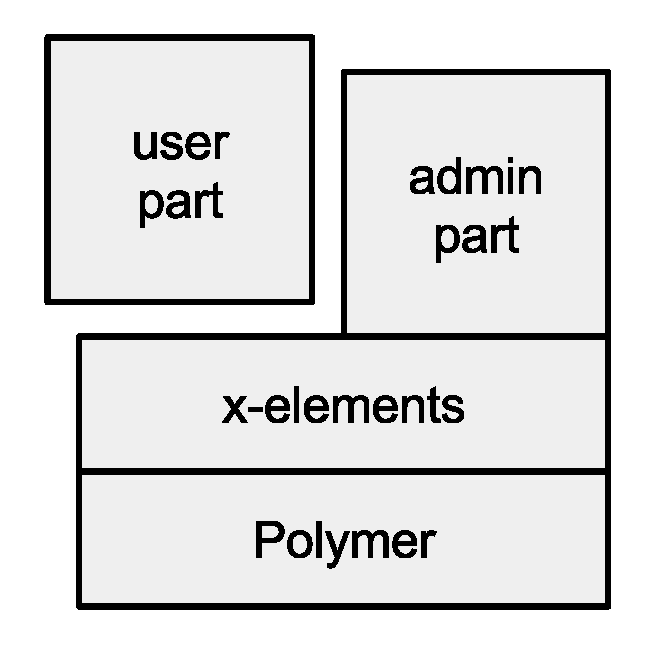
\epsfig{file=images/client-arch.eps, height=0.2\textwidth}
% \caption{Client-side architecture}
% \label{fig:client-arch}
% \end{figure}

